\documentclass[english,brazilian]{UNISINOSmonografia}
\usepackage[utf8]{inputenc} % charset do texto (utf8, latin1, etc.)
\usepackage[T1]{fontenc} 	% encoding da fonte (afeta a sep. de sílabas)
\usepackage{graphicx} 		% comandos para gráficos e inclusão de figuras
\usepackage{bibentry} 		% para inserir refs. bib. no meio do texto
\usepackage{placeins}		% float barriers
\usepackage{enumitem}

%=======================================================================
% A vantagem do unisinos.bst é que ele permite o uso de um arquivo .bib
% seguindo as orientações tradicionais do BibTeX (veja essas orientações
% em http://ctan.tug.org/tex-archive/biblio/bibtex/contrib/doc/btxdoc.pdf).
%=======================================================================
\unisinosbst

%=======================================================================
% Dados gerais sobre o trabalho.
%=======================================================================
\autor{Gräbin}{Paulo Henrique Grolli}
\titulo{Um modelo acessível de software para localização e navegação de deficientes visuais com Bluetooth Low Energy}
\orientador[Prof.~Dr.]{Costa}{Cristiano André da}
\local{São Leopoldo}
\ano{2015}

%% dados específicos para monografia de Graduação
\unidade{Unidade Acadêmica Graduação}
\curso{Curso de Bacharelado em Ciência da Computação}
\natureza{%
Trabalho de Conclusão de Curso apresentado como requisito parcial
para a obtenção do título de Bacharel em Ciência da Computação
pela Universidade do Vale do Rio dos Sinos --- UNISINOS
}

% cada palavra-chave deve ser fornecida duas vezes, uma em português e
% outra no idioma estrangeiro (na verdade, em tantos idiomas quantos se
% desejar).
\palavrachave{brazilian}{Acessibilidade Ubíqua}
\palavrachave{brazilian}{Deficiência Visual}
\palavrachave{brazilian}{Sistemas de Posicionamento Indoor}
\palavrachave{english}{Ubiquitous Accessibility}
\palavrachave{english}{Visual Impairment}
\palavrachave{english}{Indoor Positioning System}

%=======================================================================
% Início do documento.
%=======================================================================
\begin{document}
\capa
\folhaderosto

%=======================================================================
% Dedicatória (opcional).
%=======================================================================
\begin{dedicatoria}
À meus pais que sempre me incentivaram na busca por conhecimento \\e a lutar pelos meus objetivos.\\[4ex] % quebra a linha dando um espaçamento maior

\begin{itshape} % faz o texto ficar em itálico
Learning is the only thing the mind never exhausts, \\
never fears, \\
and never regrets.\\
\end{itshape}
--- \textsc{Leonardo Da Vinci} % \textsc é o "small caps"
\end{dedicatoria}

%=======================================================================
% Agradecimentos (opcional).
%=======================================================================
\begin{agradecimentos}
Agradeço primeiramente ao meu orientador Cristiano André da Costa, pessoa a quem eu muito admiro, por ter me aceito como orientando, pelas valiosas conversas, seu auxilio incomparável e por sua disponibilidade sempre que necessário.

Aos meus pais, Ivani Grolli Gräbin e Milton Gräbin, que sempre me incentivaram a estudar e a realizar meus sonhos.

A minha namorada Victoria Caroline da Silva, pela compreensão, por ficar sempre do meu lado e por me motivar a superar os desafios.

Por último mas não menos importante, aos meus amigos, os quais não diretamente ajudaram na produção desse trabalho, mas são fundamentais e estiveram do meu lado nos momentos em que necessitava esvaziar a cabeça e entendiam os convites recusados.

Muito obrigado!
\end{agradecimentos}

%=======================================================================
% Epígrafe (opcional).
%
% ``[...] o autor apresenta uma citação, seguida de indicação de autoria,
% relacionada com a matéria tratada no corpo do trabalho. Podem, também,
% constar epígrafes nas folhas de aberturas das seções primárias.''
%=======================================================================
% \begin{epigrafe}
% ``\textit{Ninguém abre um livro sem que aprenda alguma coisa}''.\\
% (Anônimo)
% \end{epigrafe}

%=======================================================================
% Resumo em Português.
%=======================================================================
\begin{abstract}
Este trabalho apresenta a modelagem de um sistema de posicionamento em ambientes internos, com recursos de acessibilidade, desenhado com o objetivo de ser usado por pessoas com deficiência visual. O modelo consiste em uma aplicação a ser usada em dispositivos móveis, utilizando beacons transmissores Bluetooth espalhados pelo ambiente para obter a localização do usuário. O sistema objetiva fornecer uma localização confiável e um deslocamento seguro através de instruções de voz, leitura de tela e feedback tátil, para permitir que seus usuários possam se deslocar em ambientes desconhecidos sem a necessidade de auxílio de outras pessoas.
\end{abstract}

%=======================================================================
% Resumo em língua estrangeira
%=======================================================================
\begin{otherlanguage}{english}
\begin{abstract}
This paper presents the modeling of a Indoor Positioning System with accessibility features, designed aiming to be used by visually impaired users. The model consists of an application to be used in mobile devices, making use of Bluetooth beacons deployed in the environment to obtain users location. The system aims to provide a reliable location and a safe and independent navigation using voice guidance, screen reading and haptic feedback in order to allow the users to navigate in unknown environments without need of assistance of other people.
\end{abstract}
\end{otherlanguage}

%=======================================================================
% Lista de Figuras (opcional).
%=======================================================================
\listoffigures

%=======================================================================
% Lista de Tabelas (opcional).
%=======================================================================
\listoftables

%=======================================================================
% Lista de Abreviaturas (opcional).
% Deve ser passada como parâmetro a maior das abreviaturas utilizadas.
%=======================================================================
% \begin{listadeabreviaturas}{seg., segs.}
% \item[ampl.] ampliado, -a
% \item[atual.] atualizado, -a
% \item[coord.] coordenador
% \item[N.~T.] Novo Testamento
% \item[seg., segs.] seguinte, -s
% \end{listadeabreviaturas}

%=======================================================================
% Lista de Siglas (opcional).
% Deve ser passada como parâmetro a maior das siglas utilizadas.
%=======================================================================
\begin{listadesiglas}{IBGE}
%\item[API] Application Programming Interface
\item[BLE] Bluetooth Low Energy
\item[GPS] Global Positioning System
\item[IBGE] Instituto Brasileiro de Geografia e Estatística
%\item[JSON] JavaScript Object Notation
\item[NFC] Near Field Communication
\item[PDV] Pessoas com Deficiência Visual
\item[RFID] Radio Frequency Identification
\item[RLSB]	Royal London Society for Blind People
%\item[SDK] Software Development Kid
%\item[SIG] Special Interest Group
%\item[SOAP] Simple Object Access Protocol
%\item[TAM] Technology Acceptance Model
%\item[TCC] Trabalho de Conclusão de Curso
%\item[UML] Unified Modeling Language
%\item[XML] Extensible Markup Language
\end{listadesiglas}

%=======================================================================
% Sumário
%=======================================================================
\tableofcontents

%=======================================================================
% Introdução
%=======================================================================
\chapter{Introdução} %Texto contextualizando o problema abordado e o escopo abarcado.
Na pesquisa bibliográfica realizada foi identificado que um grande desafio enfrentado por PDV é a localização e o deslocamento dentro de ambientes desconhecidos, tais como aeroportos, shopping centers e universidades.

O presente trabalho trata de uma alternativa para facilitar as atividades diárias das pessoas com deficiência, especialmente a visual, atuando na forma com que elas se orientam e se deslocam em ambientes internos.
Será mostrada como alternativa a modelagem de um sistema que faz uso de conceitos como dispositivos móveis, acessibilidade ubíqua, tecnologias assistivas e localização por \textit{Bluetooth Low Energy} (BLE).

Como resultado do trabalho, espera-se oferecer um sistema de fácil utilização que proporcione orientação e navegação precisas a seus usuários, de maneira que eles tenham confiança e independência. Vale ainda ressaltar que propósito do trabalho não é substituir ferramentas de auxílio como bengala e cães-guia, e sim ser um complemento a esses recursos.

	\section{Motivação}
%Texto descrevendo a motivação para o trabalho, destacando a oportunidade de pesquisa encontrada e a motivação científica. Nessa seção cabe uma figura mostrando o problema atual e como será resolvido pelo trabalho sendo realizado.

% Na introdução você deve contextualizar o problema e mostrar por que vale a pena resolvê-lo. Você deve apresentar a solução proposta e mostrar o seu diferencial em relação aos trabalhos relacionados. Observe, porém, que na introdução você deve apenas tratar do O QUÊ e PORQUÊ, sem tratar do como \cite{Hexsel11}, que deve ser explicado na seção que descreve o trabalho desenvolvido.

De acordo com o levantado por \citetexto{IBGE2010}, no último Censo Demográfico, realizado em 2010, o Brasil possuía 45,6 milhões de pessoas que afirmaram ser portadoras de deficiência. Desse total, 35,7 milhões, ou 78,2\%, são pessoas com deficiência visual (PDV). Ou seja, aproximadamente 18\% da população brasileira é afetada.

A mesma pesquisa leva em consideração as diferentes intensidades da deficiência visual, aplicando os seguintes critérios \cite{IBGE2010}: 

\begin{quote}
	Foi pesquisado se a pessoa tinha dificuldade permanente de enxergar (avaliada com o uso de óculos ou lentes de contato, no caso da pessoa utilizá-los), aplicando os seguintes critérios:
		
	• Não consegue de modo algum - para a pessoa que declarou ser permanentemente incapaz de enxergar; \\
	• Grande dificuldade - para a pessoa que declarou ter grande dificuldade permanente de enxergar, ainda que usando óculos ou lentes de contato; \\
	• Alguma dificuldade - para a pessoa que declarou ter alguma dificuldade permanente de enxergar, ainda que usando óculos ou lentes de contato; ou \\
	• Nenhuma dificuldade - para a pessoa que declarou não ter qualquer dificuldade permanente de enxergar, ainda que precisando usar óculos ou lentes de contato.
\end{quote}

Tendo diversas causas possíveis e atingindo pessoas em qualquer idade, a deficiência visual impõe severas dificuldades em todos os aspectos da vida dos que são afetados por ela. Mobilidade, educação, trabalho e vida social são exemplos, apenas para citar alguns. É difícil para uma pessoa com a visão perfeita colocar-se no lugar de uma pessoa que não enxerga. \citetexto{quinones2011supporting} afirma que mobilidade e deslocamento são atividades naturais para aqueles que enxergam sem dificuldades, podendo ir e vir com relativa facilidade, já que pistas e sinais irão apontar a direção certa caso se percam, se vejam em situações desconfortáveis ou se algum obstáculo apareça. Mostrando o outro lado, em \citetexto{URNA2007}, um trabalho que objetiva auxiliar PDV a cruzar ruas e avenidas, são citadas algumas situações usuais que são impraticáveis para PDV, como, por exemplo, ler as linhas de ônibus que passam por uma determinada parada ou ainda ler o destino de um ônibus se aproximando. Conforme \citetexto{rodriguez2014accessible}, PDV não possuem a totalidade da informação de que necessitam para contornar obstáculos. O mesmo se aplica a direção seguida e a distancia remanescente até o destino, informações essenciais para um deslocamento em ambientes desconhecidos. Não poder ver a sinalização na rua ou semáforos em um cruzamento torna perigoso para PDV transitarem desacompanhados, necessitando ter a companhia de amigos ou familiares durante todo o trajeto. Existem estabelecimentos, como, por exemplo, o metrô de Porto Alegre, que colocam uma parte de seus funcionários à disposição dos deficientes para guiá-los durante seu trajeto. Porém, seu número é limitado, o que faz com que os usuários precisem esperar até um funcionário estar disponível.

Em 2014, a Royal London Society for Blind People (RLSB), organização sem fins lucrativos que busca criar uma diferença que melhore a vida das futuras gerações de PDV, divulgou um manifesto com o resultado de pesquisas sobre perda de visão e também para chamar atenção aos desafios enfrentados diariamente, que impedem os PDV de usufruir da totalidade dos seus direitos fundamentais. Desafios esses que não são restritos às divisas do Reino Unido, onde a organização se encontra.
De acordo com o documento, perda de visão é uma experiência tão traumática que pode ser comparada à perda de um ente querido, visto que dificilmente eles recebem o apoio emocional necessário. Não conseguir ver causa isolamento social, o que prejudica enormemente o futuro do individuo. Ainda é dito que empresas ou organizações, como lojas, bancos e agentes de viagem, não compreendem as necessidades e habilidades dos PDV, impedindo-os de levar uma vida comum e impossibilitando-os de realizar as atividades que gostariam. O trabalho ainda destaca que, frequentemente, as pessoas não sabem oferecer assistência básica como guiá-los em espaços públicos como estações de trem. Dentre as áreas citadas como problemáticas, é possível destacar a mobilidade urbana, a educação superior e acessibilidade na tecnologia. A publicação trás ainda motivação que levou a sua publicação, informando que 25\% das pessoas com perda de visão estão insatisfeitas com sua vida \cite{YouthManifesto}.

Em relação à mobilidade, \citetexto{YouthManifesto} cita que existe uma variedade de aplicativos para smartphone que auxiliam pessoas a se localizar e deslocar, porém, poucos deles são acessíveis. É afirmado também que, se essas tecnologias fossem projetadas com todas as pessoas em mente, mais PDV poderiam transitar com segurança, reduzindo a dependência de outras pessoas. 

Indo ao encontro das iniciativas das RLSB e atuando na área de mobilidade, o modelo proposto visa auxiliar portadores de deficiência visual a se localizar e deslocar em ambientes internos, como, por exemplo, o campus de uma universidade, buscando facilitar o acesso à educação e à vida social disponível nos campi. Usando dispositivos móveis, o sistema irá informar ao usuário sua localização atual e recomendar caminhos que o levem ao seu destino, levando em consideração os obstáculos em sua rota.

Tendo a premissa de funcionar a partir do smartphone do usuário, o sistema será projetado para ter usabilidade intuitiva e ser uma parte quase invisível do cotidiano do usuário, aplicando o conceito de computação ubíqua introduzido em \citetexto{Weiser1991}, afim de se adaptar as necessidades dos PDV.

	\section{Questão de pesquisa}
	Como a Computação Ubíqua pode contribuir no desenvolvimento de um modelo de sistema que seja uma alternativa ao problema de localização e deslocamento em ambientes internos enfrentado por deficientes visuais, promovendo acessibilidade e permitindo o transito com confiança e independência?

	\section{Objetivos}
	Tendo identificado a questão de pesquisa, foram definidos alguns objetivos para esse trabalho, apresentados nas seções subsequentes.
	
		\subsection{Objetivo geral}
		O objetivo principal deste trabalho é especificar, desenvolver e validar um modelo de sistema para localização e orientação de PDV em ambientes internos através de dispositivos móveis, aplicando fundamentos de acessibilidade e conceitos de computação ubíqua, para permitir que seus usuários se localizem e se desloquem em ambientes desconhecidos sem necessidade do auxílio de outras pessoas.

		O sistema não deve exigir uso de hardware dedicado por parte dos usuários, devendo, porém, ser leve, discreto e de fácil uso.
		
		\subsection{Objetivos específicos}
		Para atingir o objetivo geral deste trabalho, foram definidos os seguintes objetivos específicos:

		\begin{itemize}
			\item Realizar estudo sobre deficiência visual - estudar essa deficiência buscando entender a maneira com que ela altera a vida de seus portadores e como ela afeta suas capacidades, bem como entender as necessidades que surgem a partir dela, para que os PDV possam ter uma vida mais próxima da levada pelas pessoas sem deficiência visual. Conhecer tecnologias assistivas que possam auxiliar a atingir o objetivo geral.

			\item Realizar estudo sobre computação móvel e ubíqua - compreender quais características da computação móvel e ubíqua são desejáveis em um modelo que será usado por PDV, de forma que o modelo se integre com o cotidiano de seus usuários da maneira mais natural e intuitiva possível.

			\item Realizar estudo sobre sistemas de localização e navegação - analisar trabalhos e soluções existentes nessa área, buscando entender quais características deles podem ser aproveitas em um sistema para PDV, bem como novas características que devem ser incorporadas para que as necessidades dos PDV sejam atendidas.

			\item Desenvolver um protótipo da solução - modelar e codificar uma parte do modelo proposto, criando um protótipo que utilize o conhecimento adquirido para promover um sistema que auxilie PDV e 
			possibilite a avaliação do modelo.

			\item Avaliar o sistema desenvolvido - testar o sistema com PDV e avaliar, fazendo uso de questionário, a eficácia e eficiência do sistema. O resultado ajudará identificar a aceitação, pontos fortes e possíveis melhorias do sistema, bem como elencar trabalhos futuros relacionados ao tema. (TODO: avaliação com usuários ou com estudo de caso por cenários?) 
		\end{itemize}

	\section{Organização do texto}
O presente trabalho está dividido em seis capítulos. O primeiro introduz este trabalho de conclusão de curso, bem como apresenta sua contribuição científica e objetivos.
O segundo capítulo apresenta os principais conceitos utilizados para o embasamento desde trabalho, descrevendo computação móvel e ubíqua, tecnologias assistivas, sistemas de localização e dando um panorama geral sobre a deficiência visual.
O terceiro capítulo apresenta os trabalhos relacionados feitos nesta área, cobrindo seus aspectos mais relevantes para esse trabalho, e traça um comparativo entre eles.
No quarto capítulo, é feito um detalhamento do modelo proposto neste trabalho, dando ênfase na arquitetura do sistema, seus principais requisitos e componentes que formam este modelo.
O quinto capítulo descreve a metodologia de pesquisa aplicada no trabalho, materiais utilizados e como será realizado o desenvolvimento do protótipo.
O sexto e último capítulo conclui o trabalho e apresenta as considerações finais, uma comparação com os trabalhos relacionados e sugestões de trabalhos futuros.

%=======================================================================
% Fundamentação teórica
%=======================================================================
\chapter{Referencial Teórico}
\epigrafecap{O óbvio é aquilo que ninguém enxerga, \\até que alguém o expresse com simplicidade.}{Khalil Gibran}
% Esse capítulo contém os principais conceitos e áreas envolvidos no trabalho. O capítulo deve apresentar esses conceitos em uma linha de pensamento sequencial e encadeada. Não deve conter subseções independentes sem se relacionar uma com a outra. O capítulo inícia explicando sua lógica e todas as subseções são ligadas entre si por um sequência lógica de pensamento e redação.

	\section{Computação Móvel e Ubíqua}
Tecnologias tão avançadas que deixam de ser um fim em si mesmas e passam a ser um meio para que as pessoas realizem seus afazeres. Tão conectados, tão presentes na nossa rotina e concebidas para naturalmente se integrarem em nossas vidas que deixam de ser percebidas e se colocam no plano de fundo da nossa percepção. É assim que \citetexto{Weiser1991} começa introduzindo o conceito de computação ubíqua. 

Weiser previu um mundo onde computadores deixariam de possuir apenas o tamanho de um notebook que é usado em cima de uma mesa. Um mundo onde computadores seriam pequenos o suficiente para serem embutidos em botões de uma camisa e também grandes o suficiente para ocuparem os ambientes em que convivemos, estudamos ou trabalhamos. Esses computadores conversariam entre si de maneira continua e transparente, de modo que eles e todos os usuários estariam permanentemente conectados entre si, permitindo que serviços estejam acessíveis em todos os lugares e em todos os momentos. Tal definição vai ao encontro do conceito estabelecido por \citetexto{Satyanarayanan2001} para computação móvel como sendo: “Informação na ponta dos dedos em qualquer lugar e em qualquer tempo”.

Conforme \citetexto{ballance2008developing}, a computação ubíqua oferece potencial para diminuir ou ainda eliminar as intervenções humanas necessárias em um sistema computacional.
	
	\section{Acessibilidade}

	\section{Tecnologias Assistivas}
Tecnologias assistivas tem papel chave na independência e segurança de pessoas com deficiência. Para os PDV, tecnologias assistivas bem planejadas e bem implementadas podem fazer significante diferença na educação, aceitação social e produtividade. \cite{dias2015navpal}.

Nos últimos anos tem sido feito um esforço para aumentar a acessibilidade a dispositivos e à informação disponível nestes (Ex: leitores de tela). No entanto, o mundo real apresenta muitas informações visuais, inacessível a uma pessoa cega. \cite{ucat2014}.

Em \citetexto{narasimhan2009smartphone} são sugeridos alguns princípios que devem ser seguidos no desenvolvimento de ferramentas assistivas pra PDV:
\begin{itemize}
	\item A ferramenta deve possibilitar a independência nas atividades diárias, não exigindo a assistência e/ou acompanhamento de outras pessoas, com deficiência visual ou não.
	\item Evitar adicionar melhoramentos nas bengalas, visto que aumentar o peso ou novas funcionalidades podem influenciar negativamente no uso diário
	\item Usuários devem ter a opção de usar ou não usar as funcionalidades disponíveis. Seu uso não pode ser forçado para não dificultar seu dia-a-dia.
	\item Manter custos baixos é promover a adoção de produtos pra PDV, já que produtos específicos para esse publico tendem a ser mais caros.
\end{itemize}


Diversas ferramentas existem para promover a inclusão de PDV, bem como para aliviar as dificuldades impostas pela deficiência visual. Cães-guia, bengalas e piso tátil são as principais formas usadas pra facilitar locomoção.


De acordo com \citetexto{Brady2013}, os maiores sistemas operacionais para dispositivos móveis disponíveis incluem por padrão a funcionalidade de leitura de tela, de maneira a permitir seu uso por usuários PDV. Aparelhos com tela sensível ao toque eram tidos como inacessíveis a usuários cegos, porem interfaces multitoque bem desenhadas aproveitam bem o tamanho da tela e são preferidos pelos deficientes visuais.

\citetexto{Ganz2014} destaca que smartphones são ferramentas extremamente benéficas no dia a dia das PDV, podendo ser utilizados em diversas finalidade, tais como reconhecimento de cédulas de dinheiro, objetos e cores, navegação na internet, leitura de e-mails e comunicação. O trabalho ainda afirma que o uso de smartphones é possível devido à presença de recursos de acessibilidade oferecidos pelos principais sistemas operacionais disponíveis. 

Entre esses recursos, podemos destacar a leitura de telas e os alertas vibratórios, essenciais pra aqueles que não enxergam as telas sensíveis ao toque que equipam a grande maioria dos smartphones disponíveis atualmente. Ao invés de apenas ler o texto sendo exibido, essa funcionalidade também informa sobre os tipos de cada componente, possibilitando ao usuário saber como lidar com cada um.

\citetexto{mau2008blindaid}, após pesquisa realizada em seu trabalho, define o telefone celular como “a peça de tecnologia mais valiosa para os cegos”. 

Segundo o estudo realizado por \citetexto{quinones2011supporting}, PDV possuem o desejo de carregar consigo a menor quantidade possível de equipamento. É necessário criar tecnologias que não sejam um fardo a ser carregado, mas que ofereçam a quantidade apropriada de informações ao usuário. Uma maneira citada pelo autor é a incorporação de tecnologias de navegação em aparelhos que deficientes visuais carreguem consigo normalmente, assim reduzindo o número de objetos que devem ser cuidados.
	
	\section{Sistemas de localização}

	\section{Tecnologia Bluetooth}

De acordo com \citetexto{ballance2008developing}, a combinação computação ubíqua e Bluetooth tem potencial para fomentar soluções que simples e baratas que outrora não seriam possíveis.

Bluetooth é uma tecnologia de comunicação sem fios de curto alcance, lançada comercialmente em 1990, quando teve sua primeira especificação formal divulgada. Desde então diversas modificações foram feitas e a tecnologia passou por diversos aprimoramentos, estando atualmente na versão 4.x, também conhecida como Bluetooth Smart, lançada em 2010. 

O Bluetooth foi criado e atualmente é mantido por um conjunto de empresas conhecido como Bluetooth Special Interest Group (SIG). Inicialmente formado por Ericsson, Intel, Nokia, Toshiba e IBM, o SIG é hoje composto por mais de 20.000 empresas, incluindo Apple, Microsoft, Motorola e Lenovo.

A tecnologia possui duas formas distintas de atuação, apesar de compartilharem entre si alguns pontos em comum. O primeiro e mais antigo modo, disponível desde a primeira especificação, é chamado Basic Rate (BR). O segundo foi introduzido somente na versão 4.0 e é chamado Low Energy (LE) e é o modo que será utilizado pelo modelo que será proposto.

O LE foi criado para permitir produtos que requerem baixíssimo consumo de energia e baixo custo, quando comparados ao outro modo. Assim sendo, esse modo foi pensado para aplicações que exigem pouca troca de informações. Um exemplo de produto viável com a chegada do modo LE são os beacons bluetooth, que consistem em dispositivos do tamanho de uma moeda comum, compostos por um processador, uma bateria e um transmissor, que transmitem informações sobre si em intervalos regulares. Como o sinal dos beacons tem seu alcance limitado a alguns poucos metros, foi introduzido o conceito de micro localização, tornando possível o desenvolvimento de aplicações novas aplicações e serviços onde antes não era possível, tais como lojas e pontos de venda, grandes shows ou eventos, estádios esportivos, localização em ambientes internos, etc.

A imensa maioria dos telefones celulares hoje fazem uso nativo da tecnologia, não exigindo qualquer tipo de equipamento adicional.







\citetexto{taylor2012smart} revelam que diversas tecnologias foram utilizadas anteriormente em modelos de sistema para navegação para PDV. Sonares, Radio Frequency Identification (RFID), Near Field Communication (NFC), bluetooth e Global Positioning System (GPS) são algumas dessas tecnologias. Os autores ainda apontam que apesar de todas elas oferecerem vantagens em suas propostas, todas também possuem pontos fracos:

\begin{itemize}
  \item GPS é normalmente usado para localização em ambientes externos, mas se mostra ineficiente devido à própria natureza das ondas de rádio usadas na tecnologia, quando obstáculos são locados ao redor do usuário. Além disso, GPS não é uma tecnologia ideal para ambientes internos, pois é capaz apenas de marcar um ponto em um mapa, não sendo suficiente para indicar, por exemplo, múltiplos andares em um prédio, cenário muito comum em ambientes indoor. 
  \item Sonares são formas baratas de detecção de objetos e obstáculos, através de frequências acústicas, mas exigem hardware dedicado e não servem para localização.
  \item RFID, juntamente com NFC, exige proximidade de seus emissores para que a comunicação seja estabelecida.
  \item Os autores não chegam a citar nominalmente os pontos fracos da tecnologia bluetooth, mas um grande ponto que pode ser citado é o consumo de bateria causado pelas versões que antecederam a versão 4, também chamada de bluetooth low energy.    \ldots
\end{itemize}


%=======================================================================
% Trabalhos relacionados
%=======================================================================
\chapter{Trabalhos Relacionados}
\epigrafecap{The most dangerous phrase in the language is "We've always done this way"}{Grace Hopper}

% Essa atividade consiste em detalhar os trabalhos relacionados. O capítulo começa apresentando como os trabalhos relacionados foram escolhidos. A seguir, existe uma seção descrevendo cada trabalho relacionado. Por fim, uma seção compara os trabalhos relacionados, apresentando a tabela criada na atividade 2 e descrevendo as lacunas que serão abordadas pela presente dissertação.

Para criar um novo modelo em busca de mitigar um problema enfrentado pelas pessoas com deficiência visual é necessário buscar outros trabalhos com foco na mesma área, afim de identificar falhas e virtudes de cada um, gerando um comparativo entre eles. Foram encontrados vários trabalhos que compartilham desse mesmo objetivo através do emprego de propostas tecnológicas. Neste capítulo são apresentadas 4 soluções relacionadas com o tema desse trabalho. Essas foram selecionadas por possuírem proposito semelhante bem como características desejadas por esse trabalho. Ao final desde capitulo, no item~\ref{comparacaoTrabs} é apresentado um comparativo entre os trabalhos selecionados, destacando pontos que são relevantes para o desenvolvimento da arquitetura do presente trabalho.

%=======================================================================
% PERCEPT
%=======================================================================
	\section{PERCEPT: Indoor Nagivation for the Blind and Visually Impaired}
\citetexto{Ganz2011} e \citetexto{Ganz2012} introduzem sistema de sistema de localização que busca auxiliar PDV aumentando sua percepção dos ambientes internos. O sistema é composto por um servidor central, responsável por armazenar as informações de localização do ambiente, tags RFID passivas distribuídas pelo local, leitores RFID acoplados em luvas utilizadas pelos usuários em conjunto com um smartphone Android. O principal motivo que levou a escolha do RFID é a granularidade que a tecnologia permite graças ao baixo custo de implantação e o fato de elas não exigirem fonte de alimentação elétrica. De acordo com os autores, a diferença do PERCEPT em relação a outros sistemas similares é a combinação luva/leitor e smartphone, e também o baixo custo de implantação e manutenção. 

A arquitetura do sistema também é descrita em \citetexto{Ganz2011}. Porem, \citetexto{Ganz2012} é que traz maiores detalhes. O modelo é composto pelos seguintes componentes: o ambiente, o conjunto luva PERCEPT e aplicativo Android, e por fim o servidor PERCEPT. O funcionamento deles é descrito da seguinte forma:

\begin{itemize}
	\item Ambiente é onde ficam instaladas as tags passivas de RFID. Elas podem estar dispostas de duas formas: tags comuns, colocadas em cada porta para indicar um destino específico, sempre na altura de um metro e vinte centímetros para simplificar a procura do usuário pela tag; ou então em quiosques, localizados sempre em pontos chave do ambiente, tais como entradas e saídas, elevadores ou saídas de emergência. Quiosques consistem de um conjunto de tags, que podem indicar diversos destinos possíveis, tais como salas no andar atual, diferentes andares, banheiros e saídas de emergência. É nos quiosques que o usuário informa ao sistema o destino escolhido, afim de obter a rota até ele. Em todas as tags, independentemente do tipo, está escrito o destino que ela representa, em alto relevo e em braile.
	
	\item A luva PERCEPT é responsável por obter as informações das tags através de um leitor RFID embutido. Quando a leitura de uma tag é realizada, a luva se comunica através de Bluetooth com o smartphone Android para que a rota até o destino seja calculada. O leitor é construído usando uma placa Arduino, um leitor RFID, uma antena, um chip bluetooth, uma bateria e três botões. Através dos botões o usuário pode navegar entre o conjunto de instruções da rota. De acordo com os autores, a decisão de inserir o leitor em uma luva foi tomada pois assim o usuário pode manter suas mãos livres para outras atividades. Para fazer a leitura de uma tag, o usuário deve, após encontrar aquela que contem o destino desejado entre todas as outras, posicionar a palma de sua mão com a luva em cima da tag.

	\item O aplicativo para a plataforma Android é divido em quatro módulos:
	\begin{description}
		\item[Módulo Bluetooth:] Responsável por gerenciar a comunicação com a luva PERCEPT.
		\item[Módulo Percept:] Aplicação encarregada de responder a eventos como leitura de tag e pressionamento de botões. Quando ocorre a leitura de uma tag, esse módulo manda seu identificador para o servidor, através de uma conexão sem fios, para que o cálculo da rota seja realizado.
		\item [Módulo Wifi:] Parte incumbida de estabelecer uma conexão entre o smartphone e o servidor PERCEPT.
		\item [Motor de conversão texto/voz:] Componente nativo do Android capaz de converter para voz as instruções de texto recebidas do servidor.
	\end{description}

	\item O servidor armazena o layout dos ambientes e calcula as rotas até o destino escolhido pelo usuário. Através da ferramenta Quantum GIS, cada andar é individualmente mapeado em um grafo onde cada nó representa um possível destino e cada aresta um caminho disponível. Todos os dados são armazenados em uma base de dados Postgre. O servidor calcula a rota mais curta até o destino escolhido, formulando instruções de texto, quando recebe uma requisição de um cliente Android. Uma instrução de deslocamento 

	Em uma breve avaliação do modelo, podemos ressaltar que, devido ao baixo custo das tags RFID, é fácil implantar o sistema em um grande ambiente. Porem, a necessidade de conexão constante a internet pode ser um problema. O fato de o usuário necessitar procurar os quiosques, bem como encontrar a tag correspondente ao destino desejado, é um grande contratempo.
\end{itemize}

	\FloatBarrier
	\begin{figure}[!ht]
		\caption{Arquitetura do modelo Percept}
		\label{fig:visaoGeral}
		\centering%
		\begin{minipage}{.9\textwidth}
			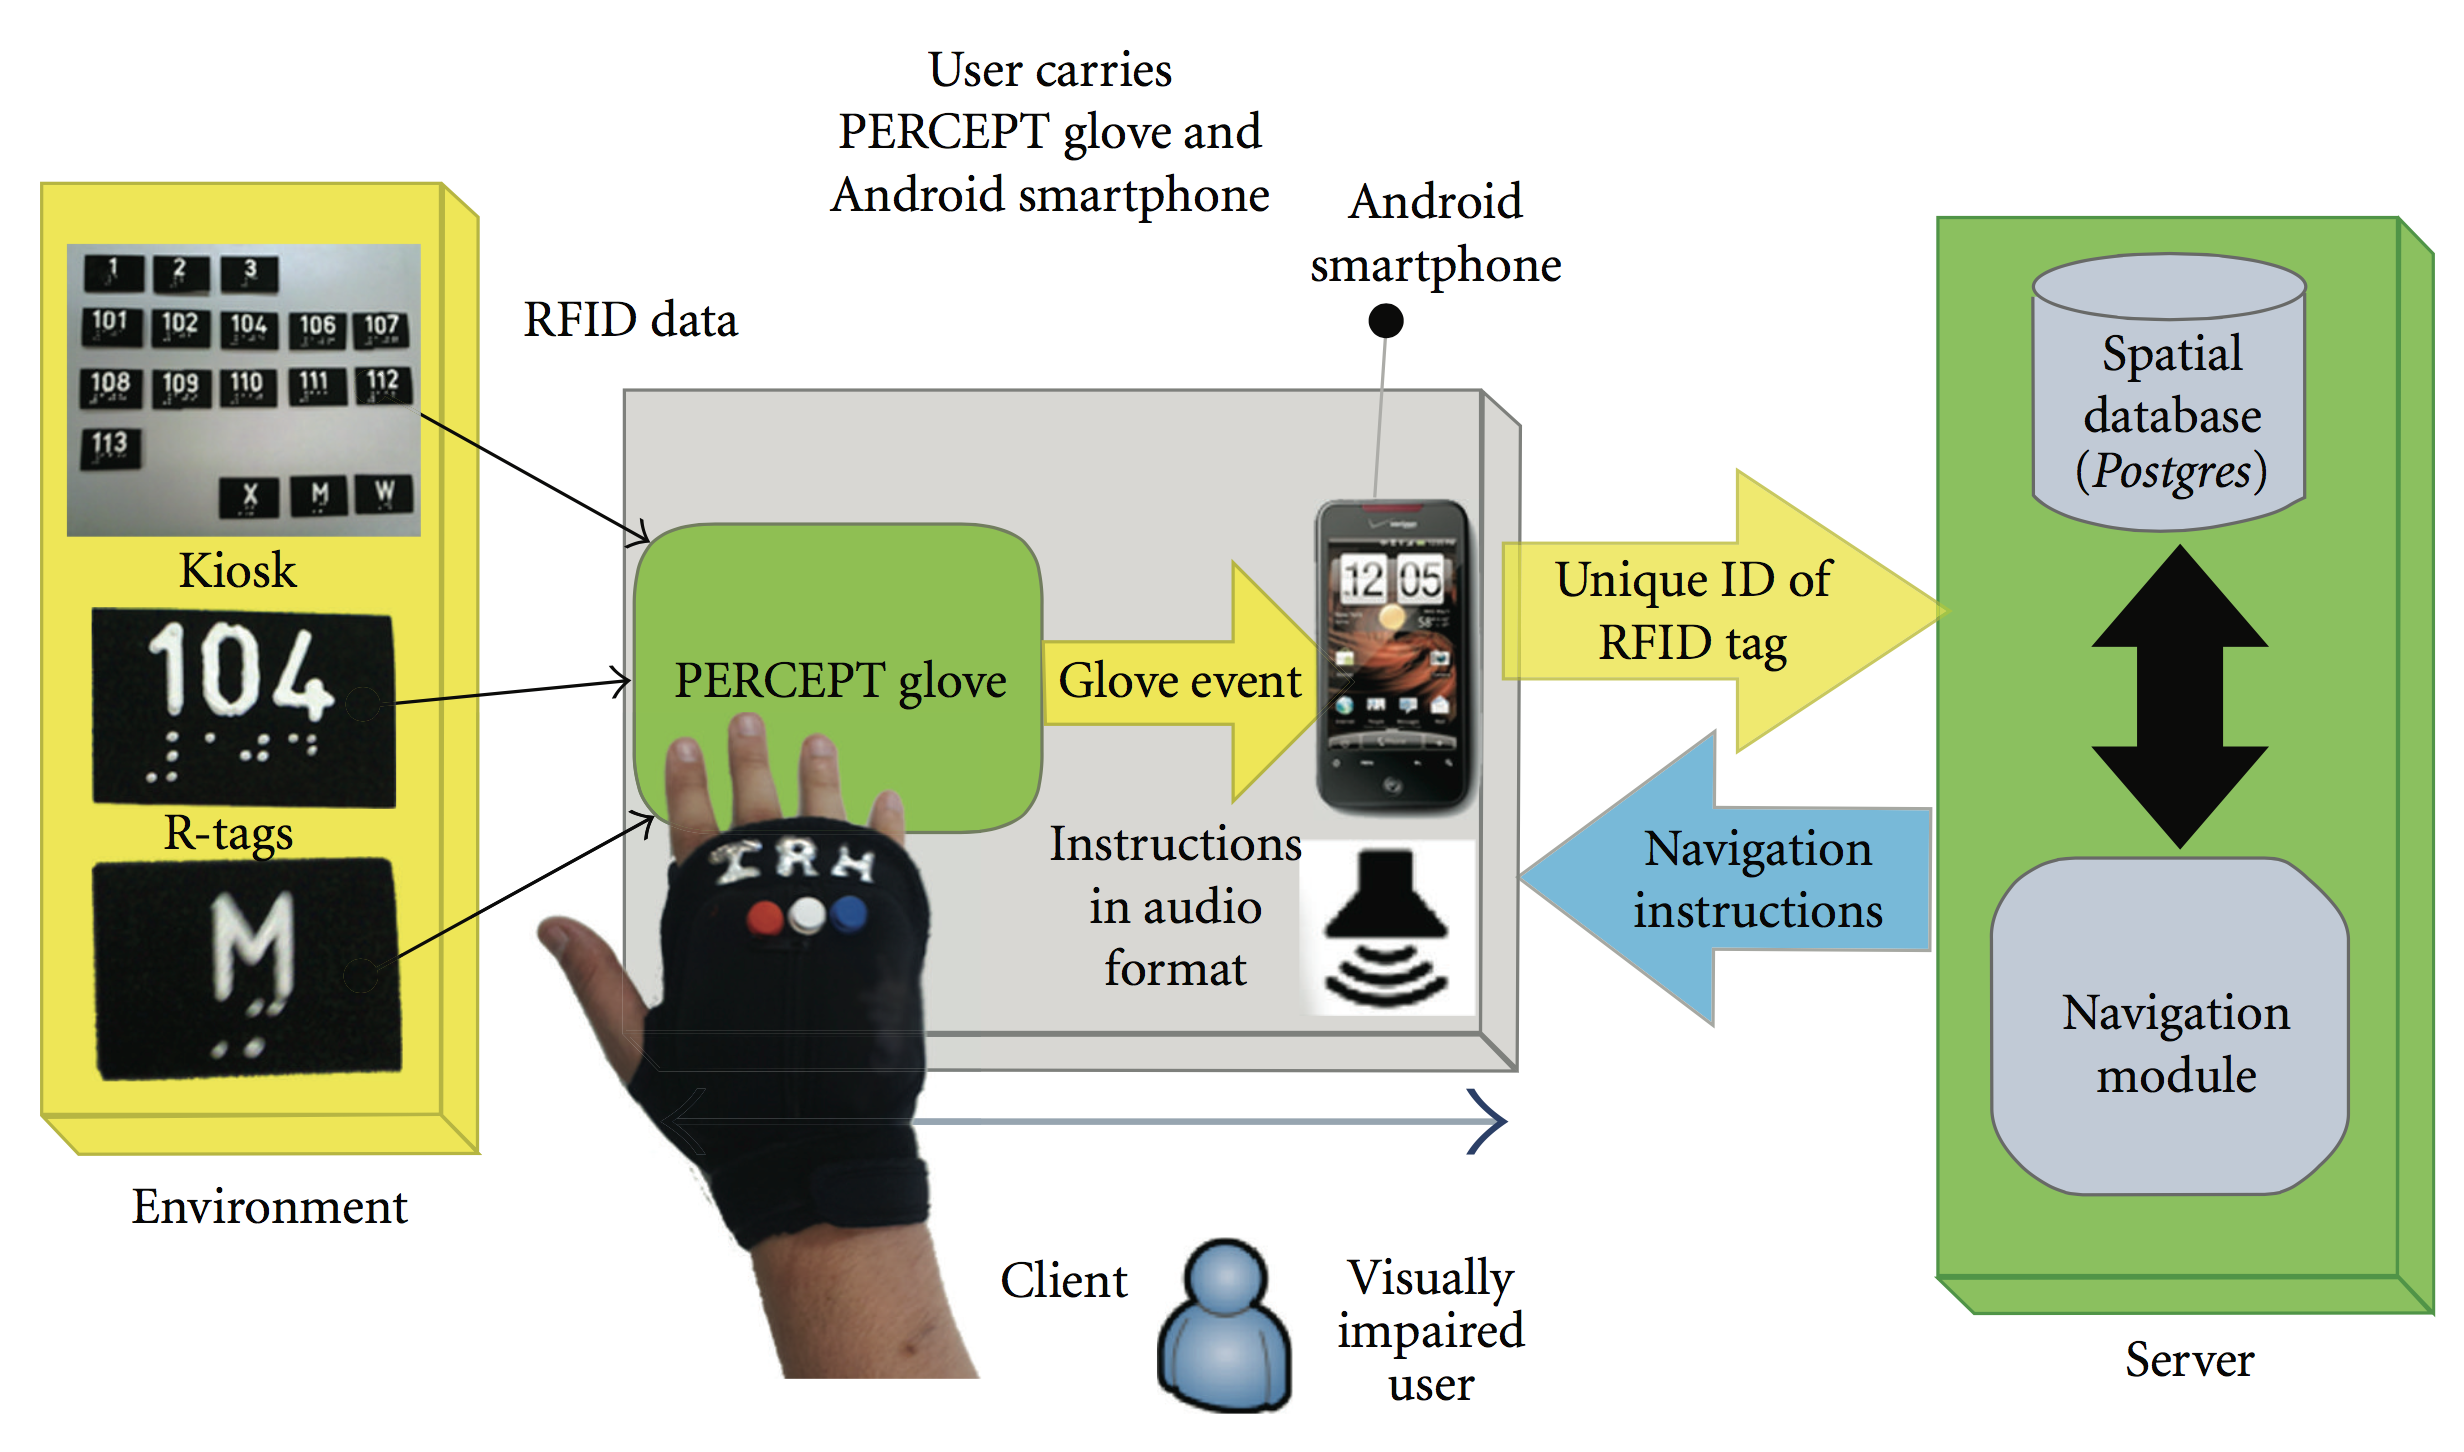
\includegraphics[width=\textwidth]{imgs/perceptArquitetura}
			\fonte{Percept}
		\end{minipage}
	\end{figure}
	\FloatBarrier

%=======================================================================
% TIRÉSIAS
%=======================================================================
	\section{Tirésias}
Em \citetexto{Falk2013} é proposto um modelo para acessibilidade chamado Tirésias. De acordo com o artigo, o Tirésias é baseado no Hefestos. Este, por sua vez, é um modelo genérico que visa procura estabelecer alguns padrões de acessibilidade que possam ser aplicados em diversos tipos de deficiência. Segundo os autores, o Tirésias pode ser compreendido como uma especialização construída em cima do modelo Hefestos para atender as necessidades das pessoas com deficiência visual. 

De acordo com \citetexto{Falk2013}, o Tirésias emprega conceitos de sensibilidade ao contexto e acessibilidade ubíqua, utilizando maneiras especializadas de interação com o sistema, para promover acessibilidade a PDV. Dessa forma, o modelo é capaz de oferecer informações relevantes ao contexto onde o usuário está e o que existe a sua volta.

O Tirésias funciona obtendo informações de localização do usuário através do GPS contido no smartphone, e, baseado nisso o sistema exibe recursos de acessibilidade disponíveis nas proximidades do usuário. Algumas das funcionalidades oferecidas são a listagem de recursos disponíveis, indicação de caminho até recurso selecionado e solicitação de ajuda.

Ainda em \citetexto{Falk2013} a arquitetura do Tirésias é descrita em seus componentes, bem como a maneira integrada em que eles operam. Os componentes citados são:

\begin{itemize} 
	\item Agente assistente pessoal
	\item Módulo de saída
	\item Módulo de entrada
	\item Módulo de configurações
\end{itemize}

\FloatBarrier
\begin{figure}[!ht]
	\caption{Arquitetura do modelo Tirésias}
	\label{fig:visaoGeral}
	\centering%
	\begin{minipage}{.6\textwidth}
		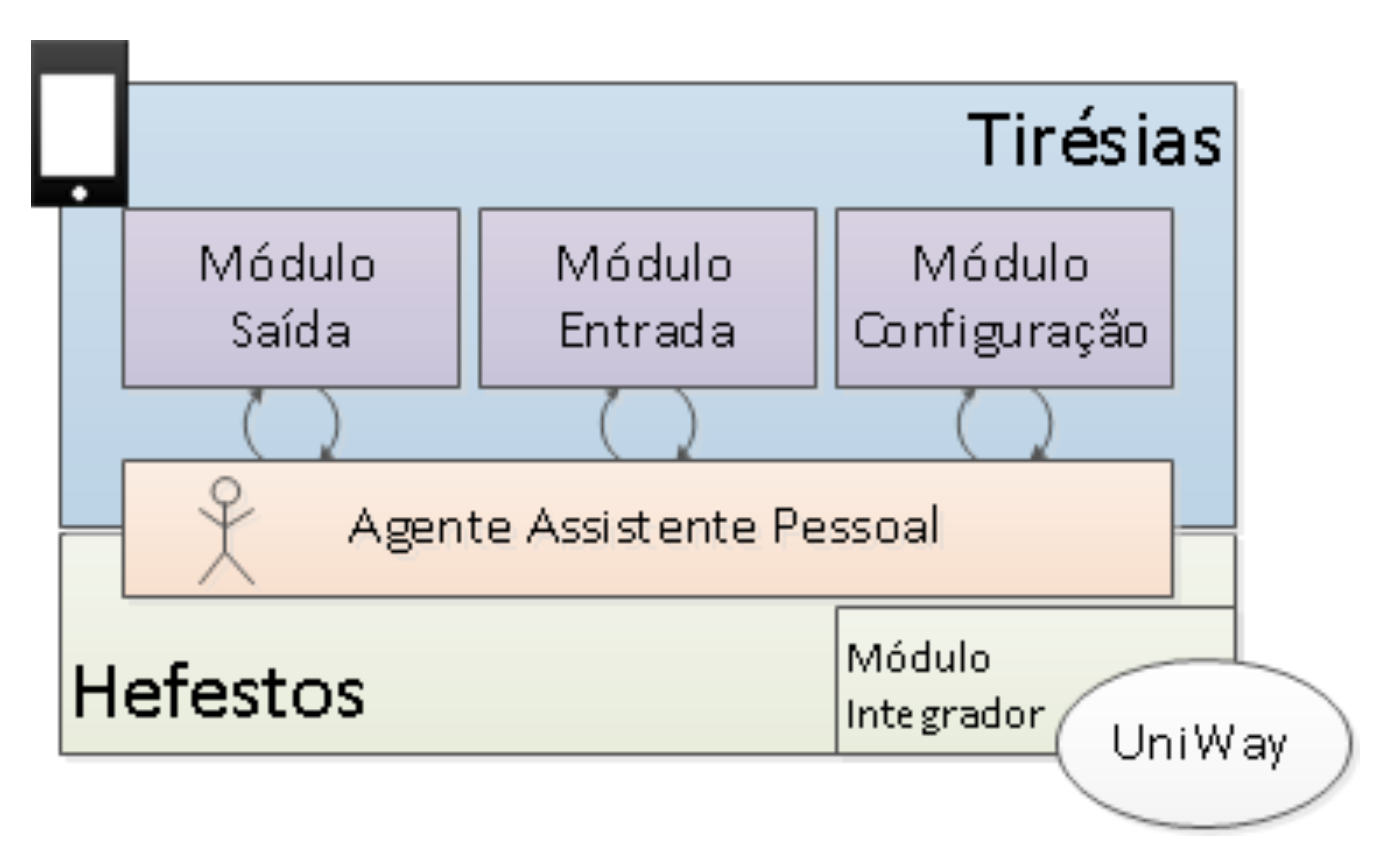
\includegraphics[width=\textwidth]{imgs/tiresiasArquitetura}
		\fonte{Tirésias: um modelo para acessibilidade ubíqua orientado à deficiência visual}
		\end{minipage}
\end{figure}
\FloatBarrier

O módulo de saída é o responsável por gerenciar as informações passadas aos usuários. Informações são dividas em dois grupos: o primeiro são indicações de recursos disponíveis próximos ao usuário; o segundo tipo são os trechos do caminho até um determinado destino escolhido pelo usuário. Para comunicar as informações ao usuário são utilizados a leitura da tela em conjunto com alertas vibratórios. A disponibilização das informações do primeiro tipo envolve a leitura do nome, da descrição e da distância até cada recurso um dos recursos disponíveis, baseado na posição atual do usuário. Conforme o usuário de movimenta, a informação de distância dos recursos é atualizada. A diferença do segundo tipo é que apenas o destino parcial mais próximo é disponibilizado, e quando o usuário concluí o trecho atual o próximo é lido. Além da leitura de tela, o Tirésias combina a utilização de alertas vibratórios com a bússola eletrônica que equipa os smartphone para indicar a direção correta aos usuários. Quando o smartphone está voltado em direção do próximo destino, o fato é informado ao usuário através de vibrações, interrompidas quando o smartphone é virado para outras direções.

O módulo de entrada gerencia a interface do usuário com o sistema. Capaz de suportar dispostívos com teclado dedicado ou somente a tela sensível ao toque, o Tirésias se adapta aos recursos disponíveis no smartphone para oferecer a maneira mais conveniente de interação ao usuário. É através deste módulo que o usuário informa ao modelo onde deseja ir, por exemplo.

O módulo de configuração disponibiliza o controle de ajustes de todas as funcionalidades disponíveis no sistema, de forma a customizar o sistema às necessidades de diferentes usuários. Alguns dos ajustes disponíveis são o controle de frequência e volume da leitura de tela, a quantidade de recursos lida e se o usuário deseja ser notificado quando há alguma mudança nos recursos.

O agente é responsável pela comunicação com o Hefestos, através da qual são obtidos perfis de usuários e recursos disponíveis para o suporte a acessibilidade. 

Avaliando o modelo, é notável a acessibilidade no que tange a entrada e saída dos dados no aplicativo. Entretanto, um ponto fraco é a utilização do GPS como modo de localização, visto que o sistema é incapaz de identificar um andar específico em um prédio com muitos pisos por exemplo, bem como o sinal pode ser fraco ou estar indisponível em algumas regiões devido a natureza da tecnologia. 


%=======================================================================
% UCAT
%=======================================================================
	\section{UCAT - Ubiquitous Context Awareness Tools for the Blind}
\citetexto{ucat2014} apresenta uma pesquisa cujo objetivo é identificar as necessidades de informação de um deficiente visual, focando principalmente em questões relacionadas...


Focando principalmente em questões relacionadas a percepção, orientação em ambientes conhecidos e desconhecidos e também em dificuldades comumente enfrentadas no dia-a-dia, após algumas entrevistas com PDV o trabalho descobriu que a falta de conhecimento a respeito das pessoas ao redor foi apontado como a principal causa de desconforto. Além disso, todos os entrevistas afirmaram que seria muito bom possuir uma ferramenta sutil e discreta que os ajudasse a obter mais informações sobre seus arredores.

O autor afirma que não existe nenhum sistema que forneça a usuários cegos informações sobre o contexto ao seu redor, e propõe um modelo com essa finalidade. Desenvolvido para dispositivos móveis que suportam a tecnologia Bluetooth, objetiva ser uma ferramenta através da qual os PDV podem criar, compartilhar e receber informações a respeito de pessoas, locais ou objetos.

O sistema usa Bluetooth para detectar pessoas próximas, relacionando contatos no smartphone do usuário com o endereço MAC do telefone dessas pessoas. A aplicação periodicamente busca dispositivos próximos, e, quando encontra algum, procura se ele foi relacionado a algum contato conhecido do usuário. Se uma relação é encontrada o aplicativo notifica o usuário através de alertas vibratórios. Aqui existe um grande ponto fraco do sistema, para funcionar corretamente 
e necessário que todos os dispositivos estevam com o Bluetooth conectado e em modo visível aos demais, caso contrário o aplicativo é incapaz de detecta-los.

A arquitetura do sistema possui estrutura cliente-servidor

\FloatBarrier
\begin{figure}[!ht]
	\caption{Arquitetura do modelo UCAT}
	\label{fig:visaoGeral}
	\centering%
	\begin{minipage}{.6\textwidth}
		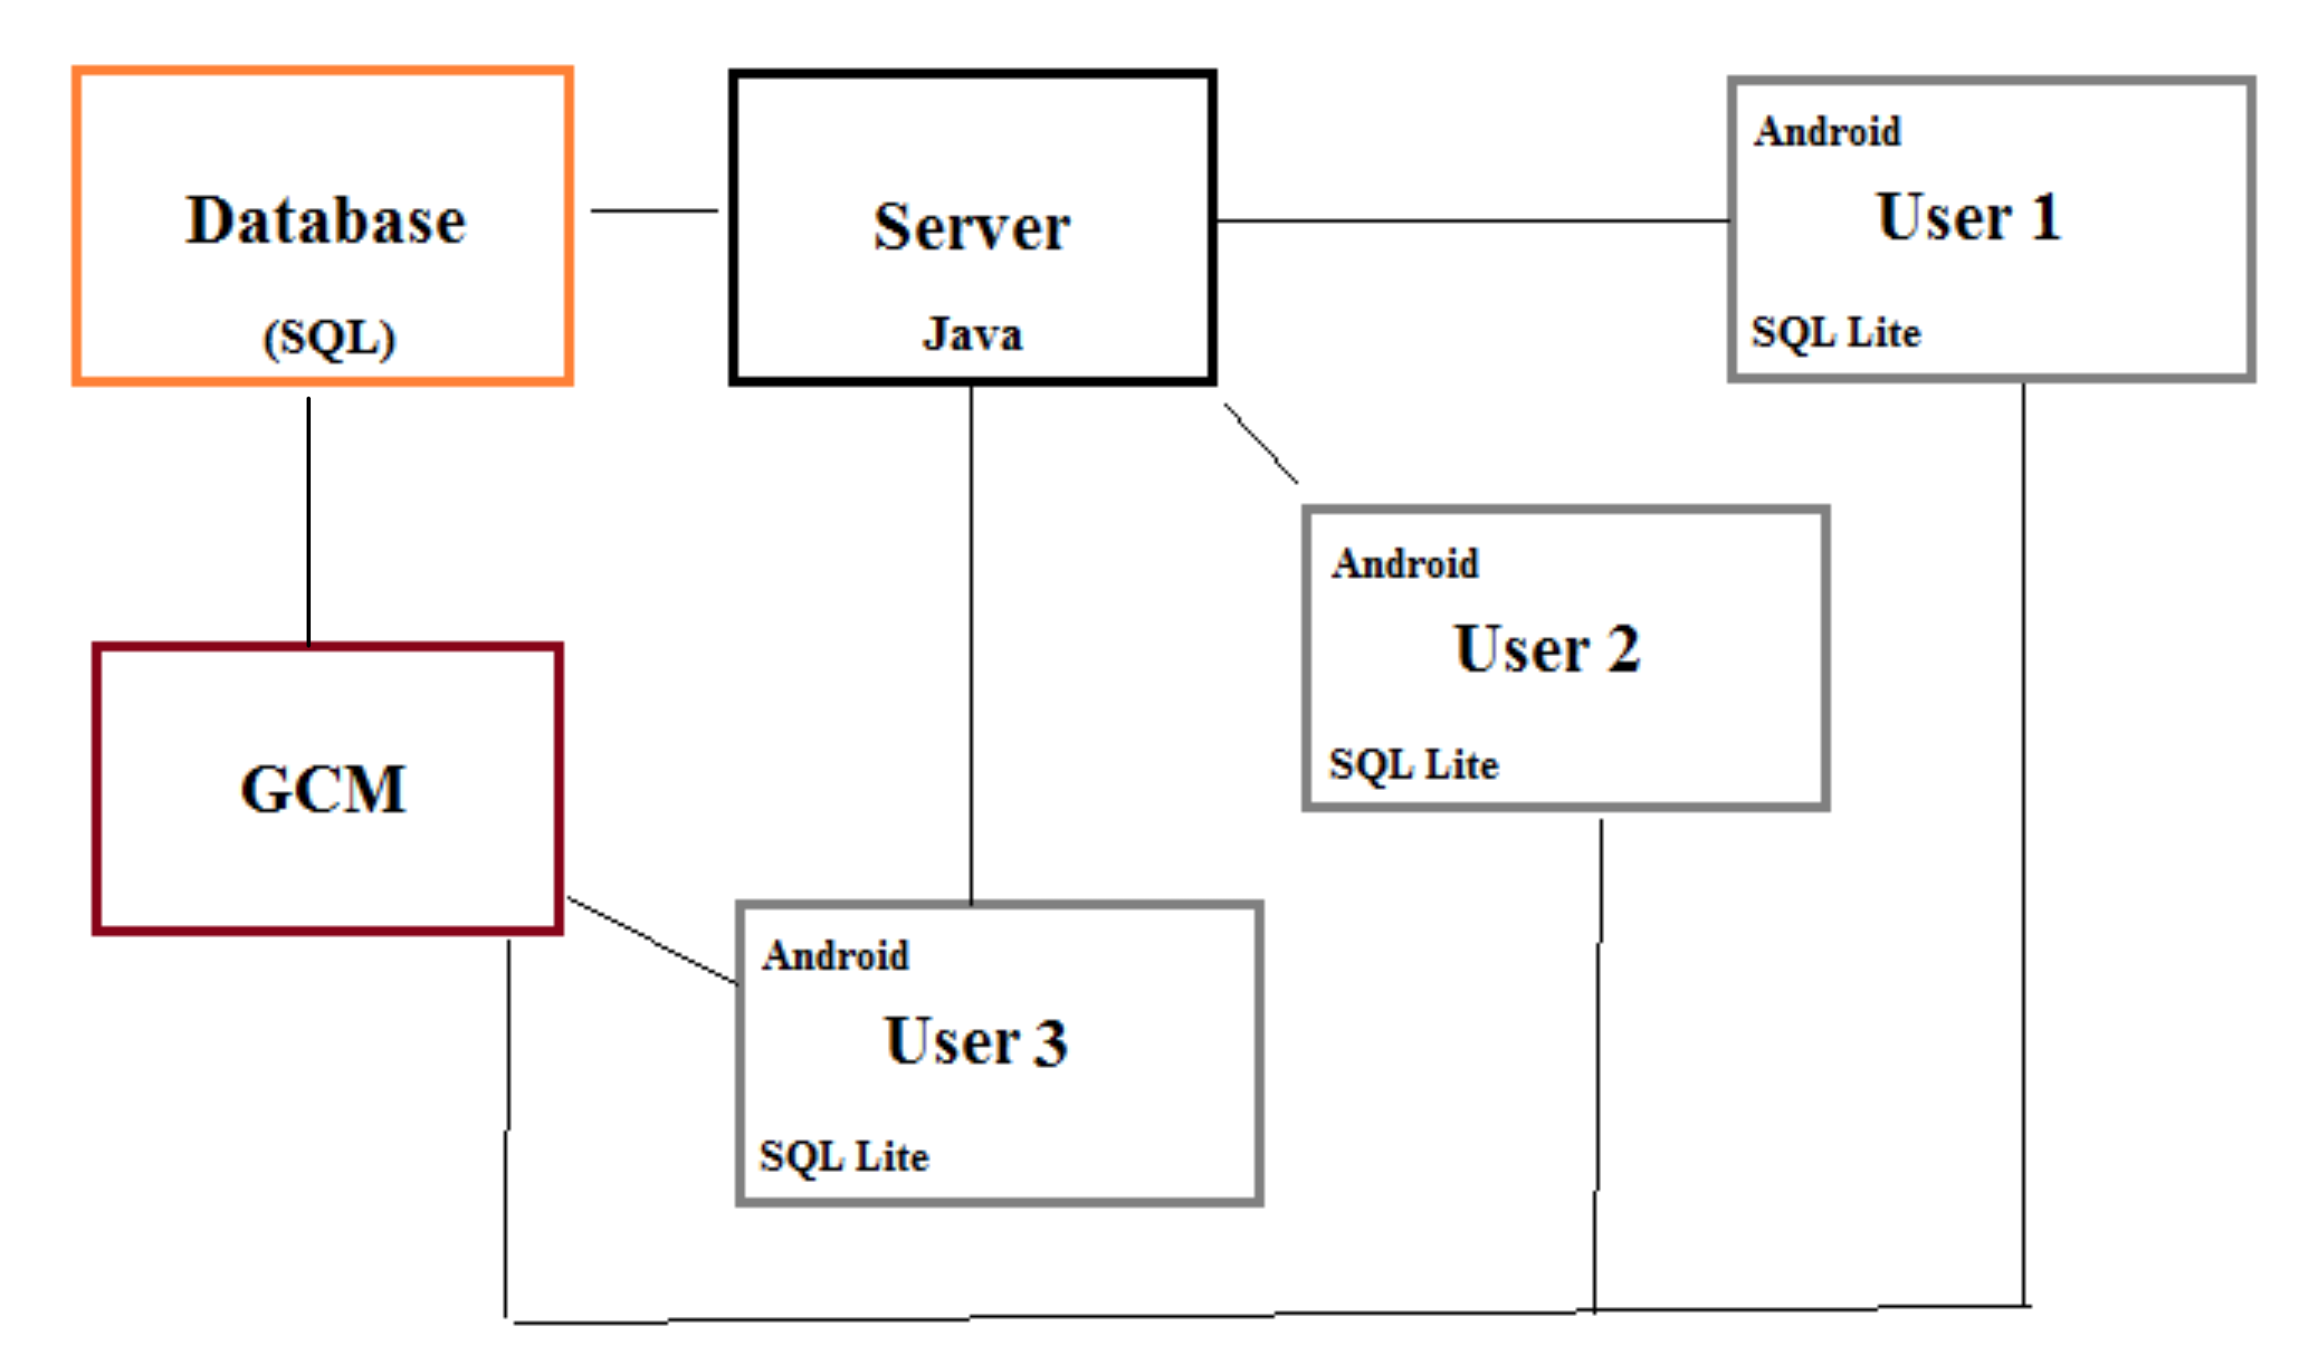
\includegraphics[width=\textwidth]{imgs/ucatArquitetura}
		\fonte{UCAT}
		\end{minipage}
\end{figure}
\FloatBarrier

%=======================================================================
% BLUETOOTH WORKZONES
%=======================================================================
	\section{Development of a Navigation System Using Smartphone and Bluetooth Technologies to Help the Visually Impareid Navigate Work Zones Safely} % (TODO: Reduzir título?)
	




	\section{Comparação entre os trabalhos estudados}\label{comparacaoTrabs}

\FloatBarrier
\begin{table}
	\caption{Tabela comparativa entre os trabalhos relacionados}
	%\label{tab:estacoes}
	\centering%
	\begin{minipage}{.6\textwidth}
		\begin{tabular*}{\textwidth}{ll}
			\hline
			\textbf{Meses} & \textbf{Estações do Ano}\\
			\hline
			21 de março a 21 de junho & Outono\\
			21 de junho a 23 de setembro & Inverno\\
			23 de setembro a 21 de dezembro & Primavera\\
			21 de dezembro a 21 de março & Verão\\
			\hline
		\end{tabular*}
		\fonte{Elaborada pela autora.}
	\end{minipage}
\end{table}
\FloatBarrier

%=======================================================================
% Modelo proposto
%=======================================================================
\chapter{Modelo Proposto}
% Essa etapa consiste em detalhar o modelo. O capítulo do modelo deve começar a partir da delimitação da pesquisa, dizendo quais lacunas serão atacadas e como. Geralmente há uma visão geral do modelo aqui, já desenvolvido na atividade 4. Esse capítulo detalha como a questão de pesquisa será respondida? Que modelo computacional é necessário para isso. Se é proposta uma ontologia, ela é detalhada aqui; Se há um modelo de contexto, ele é detalhado aqui. Pode-se usar alguns diagramas para representar a arquitetura, interações, fluxos e componentes. Lembre-se que o modelo pode ter diferentes implementações e não precisa ser limitado por uma tecnologia específica. Por exemplo, não faz sentido dizer que o modelo é para Android ou feito em Java. Por que não poderia ser para iOS e feito em Objective C? Que característica de um modelo limitaria isso?

A solução proposta através desse modelo consiste em um aplicativo acessível para dispositivos móveis compatíveis com a tecnologia Bluetooth que será usado pelos usuários, juntamente com beacons Bluetooth que fornecerão a localização do usuário. O beacons serão previamente distribuídos em pontos-chave pelo local de forma a otimizar seu alcance e área de cobertura. O aplicativo fornecerá instruções via áudio e alertas vibratórios para guiar o usuário ao seu destino, conforme o usuário for se aproximando dos beacons pelo caminho.

Este capitulo apresenta os componentes em maiores detalhes.







No Brasil, existe legislação especifica para garantir a acessibilidade e os direitos dos PDV. Os Decretos 3.298/99 e 5.296/04 definem critérios técnicos para conceituação de alguém como PDV. Os níveis de deficiência visual são baixa visão e cegueira, baseados na acuidade visual medida através de exame. A Lei 10.098/00 estabelece normas e critérios básicos para a promoção da acessibilidade, descrevendo normas de construção de edifícios públicos, de uso coletivo e privados, bem como regulamentando como deve se dar a acessibilidade nos sistemas de comunicação e sinalização. Porem, a vida digital não é contemplada pela legislação brasileira.


\citetexto{quinones2011supporting} busca entender, através de entrevistas, como PDV realizam seus deslocamentos diários, bem como elencar requisitos necessários para desenvolver sistemas que os auxiliam nesta tarefa. O trabalho afirma que PDV criam mapas mentais ricos em detalhes dos locais que mais frequentam, memorizando rotas e marcos específicos destes locais. É sugerido no trabalho que uma característica importante de um sistema para navegação é o suporte a ambientes dinâmicos, no sentido de que mesmo caminhos conhecidos podem sofrer alterações, mesmo que levemente.




Vini:
Modelo Proposto
	Visão Geral do Modelo
	Arquitetura Proposta
	Requisitos e Casos de Uso
		Requisitos Funcionais
		Requisitos Não Funcionais
	Modelo do Prontuario Proposto


Plets:
Modelo Proposto
	Requisitos
		Requisitos Funcionais
		Requisitos Não Funcionais
	Arquitetura
	Modelo de Dados
	Modelo de Segurança
		Senha
		Identificação de uso indevido
		Criptografia
	Modelo de comunicação
	Modelo de contexto


	\section{Visão Geral}

A Figura~\ref{fig:blablabla} mostra ilustra as fases psicológicas da escrita da dissertação. Você vai se reconhecer no personagem. ;-)

\FloatBarrier
\begin{figure}[!ht]
	\caption{Visão geral do modelo}
	\label{fig:blablabla}
	\centering%
	\begin{minipage}{.8\textwidth}
		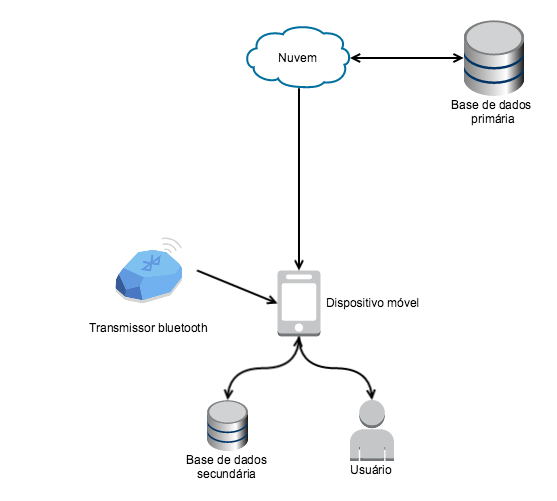
\includegraphics[width=\textwidth]{imgs/visaoGeral}
		\fonte{Elaborado pelo autor.}
	\end{minipage}
\end{figure}
\FloatBarrier

	\section{Requisitos}

	\section{Arquitetura}
 

\FloatBarrier 
\begin{figure}[!ht]
	\caption{Diagrama de blocos da arquitetura}
	\label{fig:arquitetura}
	\centering%
	\begin{minipage}{.8\textwidth}
		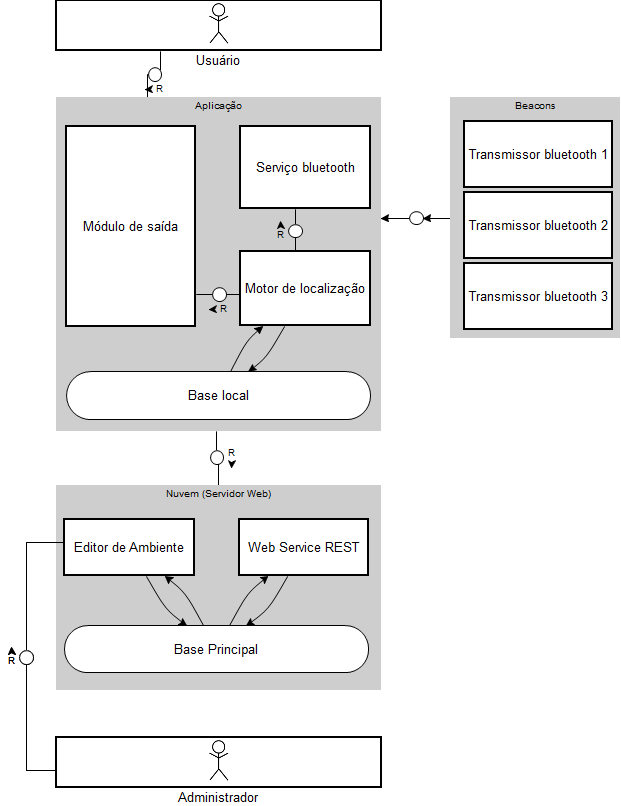
\includegraphics[width=\textwidth]{imgs/arquitetura.png}
		\fonte{Elaborado pelo autor.}
	\end{minipage}
\end{figure}
\FloatBarrier 




%=======================================================================
% Metodologia
%=======================================================================
\chapter{Metodologia}
Enquadrando o presente trabalho na classificação apresentada em \citetexto{Gerhardt2009}, quanto à natureza da pesquisa, ele se caracteriza como uma pesquisa aplicada, pois objetiva gerar conhecimentos para aplicação prática dirigidos a solução de um problema específico que é a navegação e localização de deficientes visuais. A abordagem do trabalho é qualitativa e, do ponto de vista dos objetivos, é uma pesquisa exploratória e descritiva, buscando resultar em um modelo acessível de localização e navegação em ambientes internos. O procedimento técnico utilizado para a construção da pesquisa é a pesquisa bibliográfica.

	\section{Desenvolvimento}
O trabalho de modelagem de desenvolvimento do xxxxxxx (TODO) foi divido em (TODO) XX passos metodológicos apresentados na figura (TODO) XX. Os passos 1 a X foram realizados no presente trabalho. Os demais passos serão realizados na disciplina Trabalho de Conclusão II, que também compreende os requisitos para a colação de grau da Universidade do Vale do RIo dos Sinos (UNISINOS).

A seguir são apresentados brevemente cada um dos passos concebidos:

% passos
\begin{enumerate}
	%	1
	\item \textbf{Revisar bibliografia:} blablabla
	%	2
    \item \textbf{Realizar estudo sobre deficiência visual:} blablabla
	%	3
    \item \textbf{Realizar estudo sobre sistemas de localização e navegação:} blablabla
	%	4
    \item \textbf{Realizar estudo sobre tecnologias assistivas:} blablabla
	%	5
    \item \textbf{Realizar estudo sobre computação móvel e ubíqua:} blablabla
    %	6
    \item \textbf{Elencar requisitos e modelar o sistema:} blablabla
    %	7
    \item \textbf{Codificar sistema:} blablabla
	%	8
	\item \textbf{Testar aceitação do sistema:} blablabla	
	%	9
	\item \textbf{Analisar resultados dos testes:} blablabla
\end{enumerate}

	\section{Avaliação}
A avaliação do modelo proposto se dará após a implementação e implantação do sistema. Para a implantação do mesmo serão convocados usuários PDV com interesse em colaborar com a pesquisa. Os usuários utilizarão o sistema e posteriormente o avaliarão usando duas técnicas distintas. A primeira será através de questionários anônimos durante o período de testes, afim de detectar problemas pontuais e verificar a adaptação do usuário ao sistema durante o período de uso. A segunda será a técnica da entrevista estruturada. 

A entrevista ocorrerá em dois momentos. Antes de iniciar o período de testes para obter informações sobre a forma como os usuários se guiam quando necessitam deslocar-se em um ambiente desconhecido. Após o termino dos testes para obter informações relativas a qualidade da localização e da navegação oferecida pelo protótipo. O resultado da analise permitirá identificar a eficácia do sistema e possibilitará elencar melhorias e/ou trabalhos relacionados ao tema.

(TODO avaliação por cenários ou usuários)

\chapter{Conclusão}

\section{Comparação entre os trabalhos estudados e o modelo proposto}

	\begin{table}
		\caption{Comparação entre os trabalhos estudados e o modelo proposto}
		%\label{tab:estacoes}
		\centering%
		\begin{minipage}{.6\textwidth}
			\begin{tabular*}{\textwidth}{ll}
				\hline
				\textbf{Meses} & \textbf{Estações do Ano}\\
				\hline
				21 de março a 21 de junho & Outono\\
				21 de junho a 23 de setembro & Inverno\\
				23 de setembro a 21 de dezembro & Primavera\\
				21 de dezembro a 21 de março & Verão\\
				\hline
			\end{tabular*}
			\fonte{Elaborada pela autora.}
		\end{minipage}
	\end{table}
	
	\section{Trabalhos futuros}
- Ambientes dinâmicos
- Salas de aula

Em caso de dúvida, siga as orientações do manual da Biblioteca \cite{Biblioteca11} e, se necessário, da norma NBR~6023 \cite{NBR6023:2002}.


























































Geralmente, a introdução tem uma estrutura similar ao resumo e deve apresentar:
\begin{itemize}
	\item \textbf{Contexto e motivação:} Aqui você deve apresentar o contexto do trabalho (área de que ele se trata) e uma motivação para trabalhar nesse assunto.
	\item \textbf{Problema:} Aqui você vai apresentar um problema, uma lacuna, observada na área e que você pretende tratar. Você deve se perguntar aqui: ``Que respostas estou disposto a responder?''. O problema deve ser definido claramente e delimitado em termos de espaço de tempo. Veja que essa parte visa alertar o leitor de que o que você está propondo é uma solução para um problema observado na área. 
	

	\item \textbf{Objetivos:} Aqui você deve apresentar os objetivos do seu trabalho. Tome cuidado para não confundir objetivos com atividades.   Faça a si mesmo a pergunta: ``O que pretendo alcançar com a pesquisa?''. Você pode discernir entre objetivos gerais e objetivos específicos:
	\begin{itemize}
		\item Objetivo geral --- qual o propósito da pesquisa?
		\item Objetivos específicos --- abertura do objetivo geral em outros menores (possíveis capítulos).
	\end{itemize}
	
\end{itemize}

%=======================================================================
% Referências
%=======================================================================
\bibliography{bibliografia}

\end{document}